\documentclass{article}

\def\summary{
%%%%%%%%%%%%%%%%%%%%%%%%%%%%%%%%%%%%%%%%%%%%%%%%%%%%%%%%%%%%%%%%%%%%%%%%
This report summarizes work done as part of the Visualizing Large Data Sets PFUG under Rice University's VIGRE program.  VIGRE is a program of Vertically Integrated Grants for Research and Education in the Mathematical Sciences under the direction of the National Science Foundation.  A PFUG is a group of Postdocs, Faculty, Undergraduates and Graduate students formed round the study of a common problem.  This module will do exploratory analysis on large data sets, specifically data related to the housing crisis.
%%%%%%%%%%%%%%%%%%%%%%%%%%%%%%%%%%%%%%%%%%%%%%%%%%%%%%%%%%%%%%%%%%%%%%%%
}

\usepackage{html}
\usepackage{cite}
\usepackage{graphicx}


\begin{document}
%%%%%%%%%%%%%%%%%%%%%%%%%%%%%%%%%%%%%%%%%%%%%%%%%%%%%%%%%%%%%%%%%%%%%%%%%%%%%%%%

\section{Introduction}

The US housing crisis has undermined the world economy in wide reaching and poorly understood ways. Although there is a lot of speculation over the causes and the effects of the housing crisis, most of these ideas come from opinionated blogs or news articles that do not list their sources.  This lack of data becomes perilous as the US government invests trillions of dollars based on untested hypotheses concerning the crisis.  Our PFUG's focus is to compile, clean, and analyze data pertaining to the housing crisis to get a clearer picture of what is actually going on.  

\section{Overview and Motivation}

\subsection{Real Estate Bubble:} Around 2006, house prices rose much higher than their true value. Eventually, housing prices became so high, it was difficult for current owners to afford their house. As foreclosure rates increased, house prices began to plummet. This has largely affected the global economy. 
\subsection{Little Public Organized Data:} There is a lot of speculation over the causes and the effects of the housing crisis. Unfortunately, most of these ideas come from opinionated blogs or news articles that don�t list their sources. Therefore, it is difficult to collect reliable information.
\subsection{Government Expenditures:} The government has already exhausted millions of dollars in order to aid those affected by housing crisis. With such little public data about the crisis, we are left wondering what data the government is using.  
\subsection{Still Unfolding:} It is important to realize that the housing crisis in ongoing. This allows us to track its progression and hopefully make predictions for the upcoming years. 
\subsection{Large Data Sets:} The housing crisis serves as a perfect model for visualizing large data sets. Most data sets we collect usually cover multiple years, counties and variables. 


\section{Problems with Large Data}

\subsection{Hard To Find} All of the data we have collected come from multiple sources. Currently, there is no central repository where data can be found.  
\subsection{Licenses and Fees} Some of the data sets have licenses that do not allow us to reproduce or publish any of our findings. Also many of the data sets cost large amounts of money to purchase. 
\subsection{Size} Some data sets were as large as 10 GB. In order to work around this problem, we were able to extract certain parts of the data sets without having to completely download them. 
\subsection{Dirty} Most of the data sets we find are what we call �dirty.� They are usually unorganized and practically unreadable.  



\section{Data Sets}
To view our most current data sets and work, please visit our PFUG's website on \htmladdnormallink{Github}{http://github.com/hadley/data-housing-crisis/tree}.
Some of our major data sets include \ldots
\begin{itemize}
\item American Community Survey
\item Case-Shiller House Price Index (HPI)
\item Census 2007
\item Construction of Housing Units
\item Market Value of 1 month rent in a Room
\item Vacancies 
\item Mortgage Rates
\item Federal Housing Finance Agency HPI
\end{itemize}


\section{Cleaning and Analysis}
To facilitate sharing data, we have conducted both data cleaning and analysis with the open source statistical software R, which is available free of charge at \htmladdnormallink{R-Project}{http://www.r-project.org}.  We use  the program R to clean our data sets. R is considered a statistical standard among statisticians. There are several advantages to using R. We are able to manipulate extremely large data sets ( \textgreater 2GB) on a normal desktop. It also allows us to produce impressive graphics with minimal coding.

\subsection{Clean Data is\ldots}\label{cleandatais}
\begin{itemize}
\item \textbf{Consistent:} In a few data sets county names change over the course of a few years. This affects how we compare yearly data.
\item \textbf{Concise:} Some data sets contained only parts of information we needed. For example, the American Community Survey contains over 200 questions. We were only interested in the answer to one of those questions. 
\item \textbf{Complete:} One of the data sets that was collected  was missing around 80\% of the data. 
\item \textbf{Correct:} We must assume that the data we collect is not corrupt and was recorded properly. Some smaller data sets contained unusual observations. We used our own discretion when deciding what data sets were correct. 
\end{itemize}

\subsection{Cleaning Process}

\begin{enumerate}
\item First we start with ``dirty'' data. (Fig. \ref{fig:dirtydata})

\begin{figure}[htp]
\begin{centering}
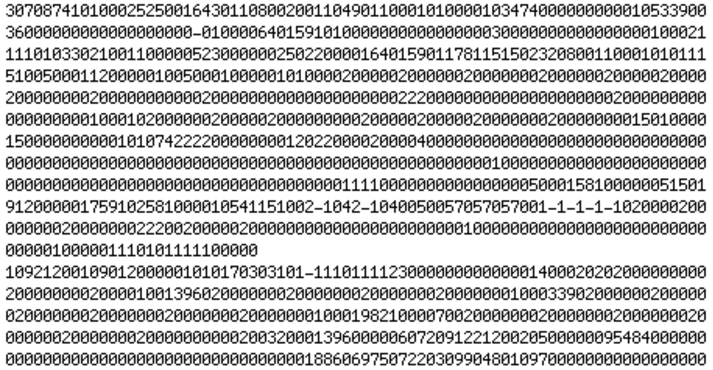
\includegraphics[scale=1]{download.pdf}
\caption{Snapshot of ``dirty'' data.}
\label{fig:dirtydata}
\end{centering}
\end{figure}

\item Next we must download the data.  A section of download code is shown below. (Fig. \ref{fig:dirtydataR})

\begin{figure}[htp]
\begin{centering}
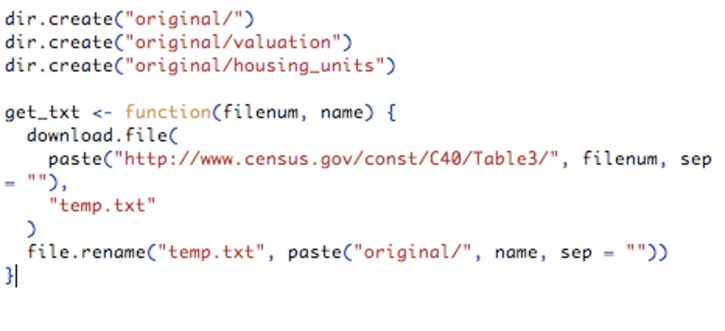
\includegraphics[scale=1]{download-r.pdf}
\caption{Snapshot of R code to download the ``dirty'' data.}
\label{fig:dirtydataR}
\end{centering}
\end{figure}

\item Once we have the data, we clean the data as best we can according to the rules in ``Clean Data Is\ldots''(Sect. \ref{cleandatais}). A section of cleaning code is shown below. (Fig. \ref{fig:cleanR})

\begin{figure}[htp]
\begin{centering}
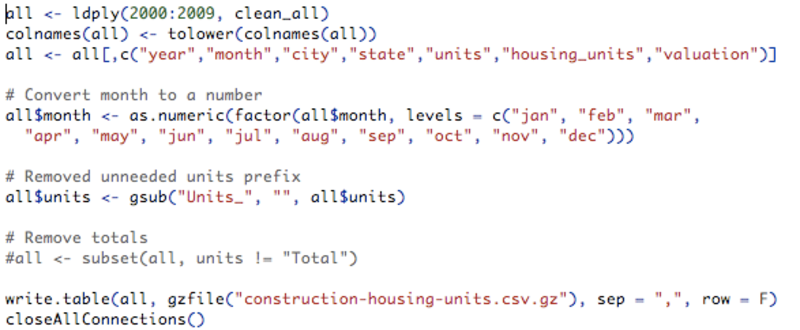
\includegraphics[scale=1]{clean-r.pdf}
\caption{Snapshot of R code to clean data.}
\label{fig:cleanR}
\end{centering}
\end{figure}

\item Now that the data has been cleaned, it may look like the top part of the data below. (Fig. \ref{fig:clean})

\begin{figure}[htp]
\begin{centering}
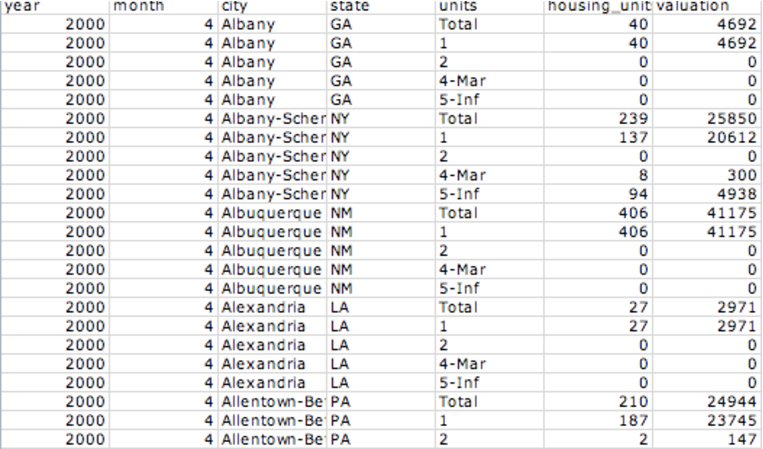
\includegraphics[scale=1]{clean.pdf}
\caption{Snapshot of ``clean'' data.}
\label{fig:clean}
\end{centering}
\end{figure}


\item With clean data, we are able to explore it.  The code below (Fig. \ref{fig:vizR}) is the command used to produce the plot in figure Fig. \ref{fig:viz}.

\begin{figure}[htp]
\begin{centering}
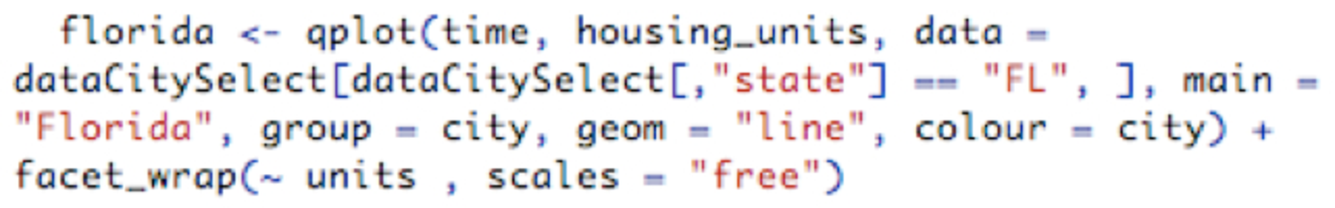
\includegraphics[scale=.5]{vizfl.pdf}
\caption{Snapshot of R code to produce exploratory graphics.}
\label{fig:vizR}
\end{centering}
\end{figure}

\item With R code we are able to produce complex plots with minimal amount of code. (Fig. \ref{fig:viz})

\begin{figure}[htp]
\begin{centering}
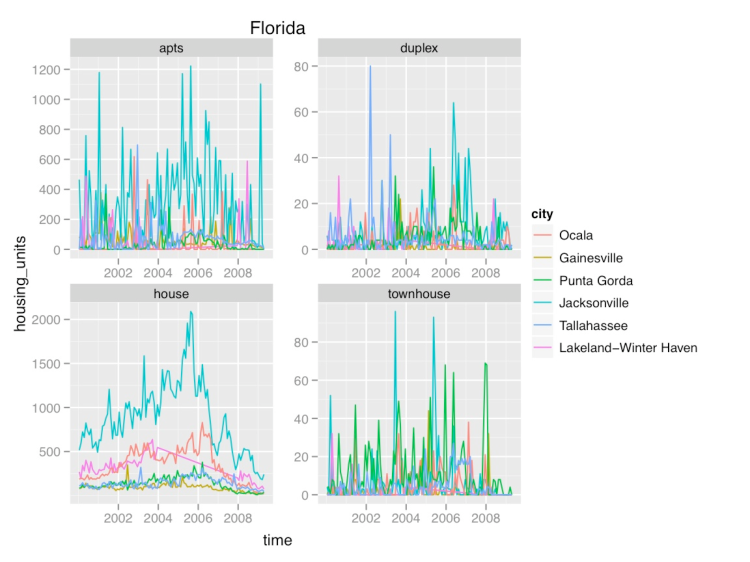
\includegraphics[scale=1]{viz.pdf}
\caption{Example graphic.  Exploring construction data in Florida.}
\label{fig:viz}
\end{centering}
\end{figure}



\end{enumerate}



\section{Interesting Findings}

\subsection{Location, Location, Location...}

The data graphed (Fig. \ref{fig:usatime} \& Fig. \ref{fig:hpitime}) is from the Federal Housing Finance Agency (FHFA) house price index (HPI). Both of these graphs analyze what time the HPI peaked for each metropolitan statistical area (MSA). 

Looking at both graphs we believe that timing seems to be very significant. If a state peaked earlier than 2006 or later than 2007, their HPI was not as greatly affected. This also supports the claim that California and Florida were impacted the greatest.

In Figure \ref{fig:usatime}, you can see that both California and Florida peaked around the same time.  

In Figure \ref{fig:hpitime}, every point is a MSA and labeled by state. It graphs the peak HPI time versus the percent change in HPI between then maximum HPI to 2009, quarter 1 HPI. This graph shows that if HPI peaked between 2006 and 2007, then that state typically experienced a much larger percent change in HPI. 

\begin{figure}[htp]
\begin{centering}
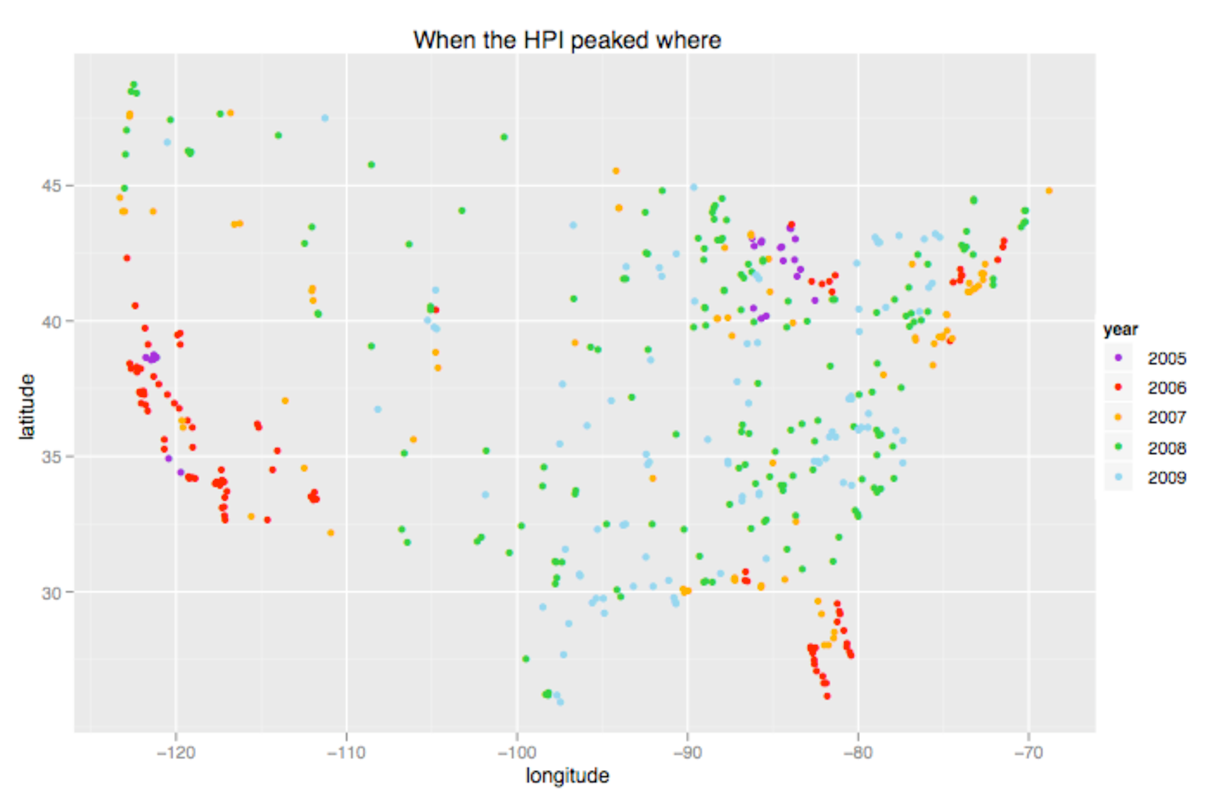
\includegraphics[scale=0.5]{usatime.pdf}
\caption{Graphs what year each MSA area reached their maximum housing price index.}
\label{fig:usatime}
\end{centering}
\end{figure}

\begin{figure}[htp]
\begin{centering}
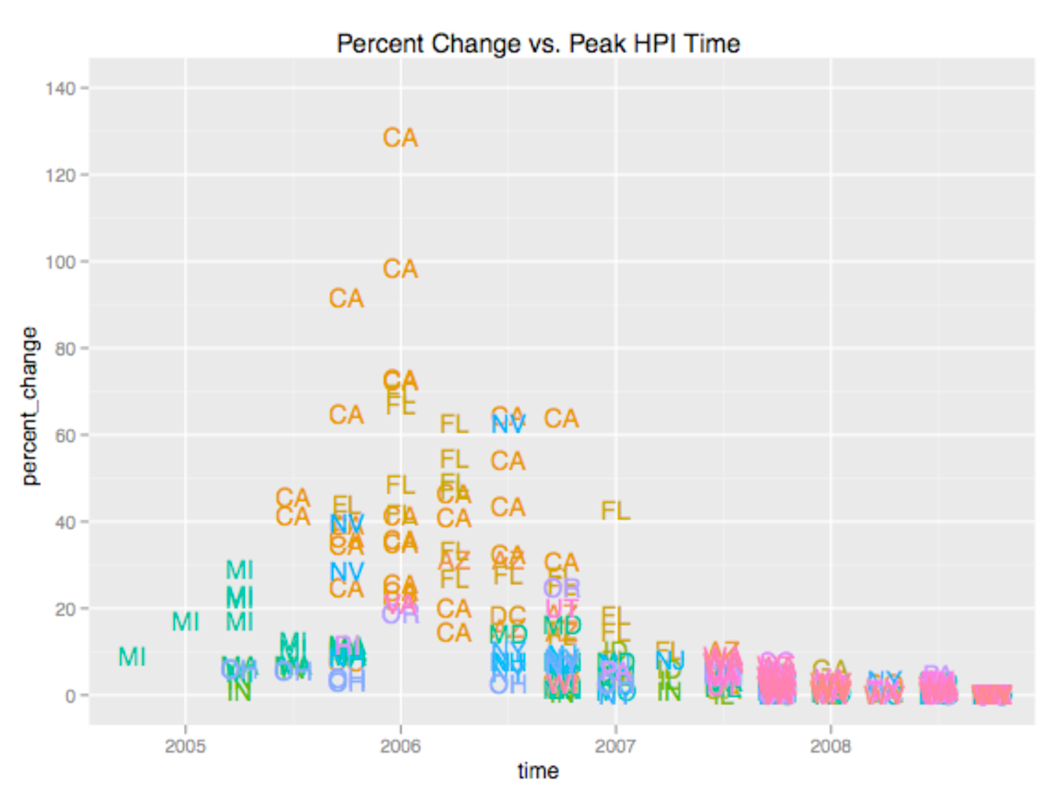
\includegraphics[scale=0.5]{hpitime.pdf}
\caption{Graph showing the percent difference between the maximum housing price index and the 2009 housing price index plotted against the time in which the maximum housing price index occurred.}
\label{fig:hpitime}
\end{centering}
\end{figure}


\subsection{Merced, CA}

The city with the greatest percent change in the FHFA HPI was Merced, CA. This observation is very unusual of small cities. Further research into Merced showed that University California of Merced has finished construction in late 2005. Using both Figure \ref{fig:merchpi} and \ref{fig:merccon}, we hypothesize that the construction increased due to the necessity of housing for UC Merced students and employees. 

\begin{figure}[htp]
\begin{centering}
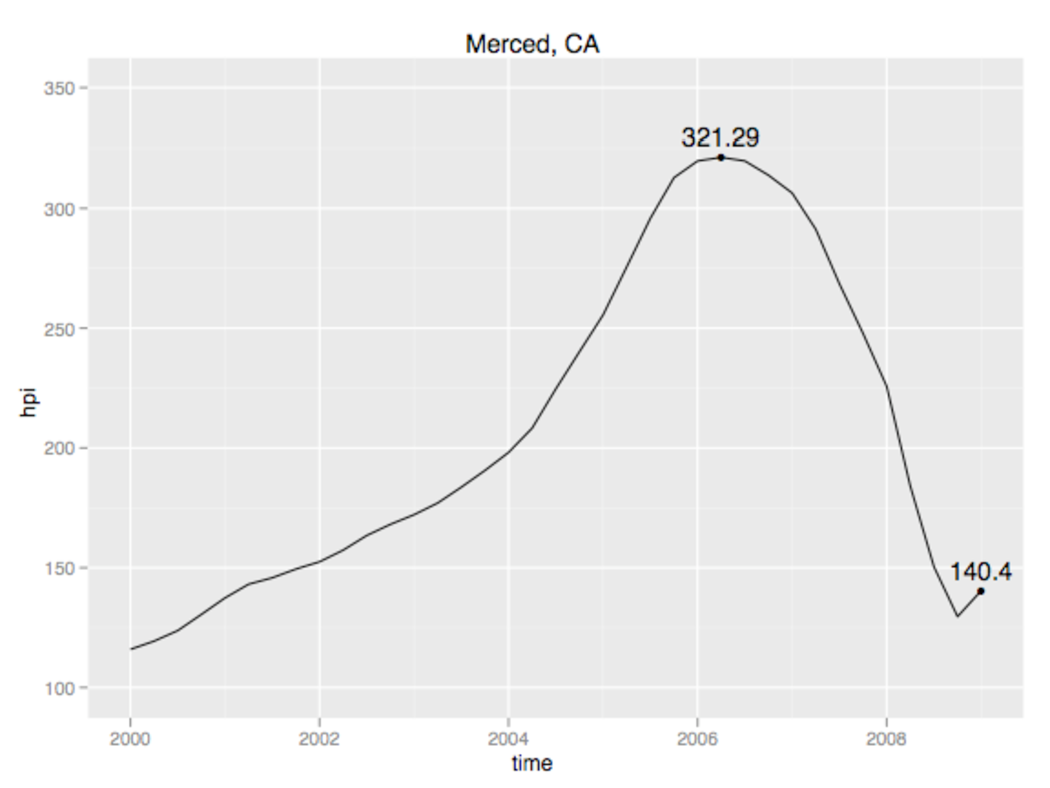
\includegraphics[scale=0.5]{merchpi.pdf}
\caption{Merced, California's housing price index over time, with the maximum and 2009 time points highlighted.}
\label{fig:merchpi}
\end{centering}
\end{figure}

\begin{figure}[htp]
\begin{centering}
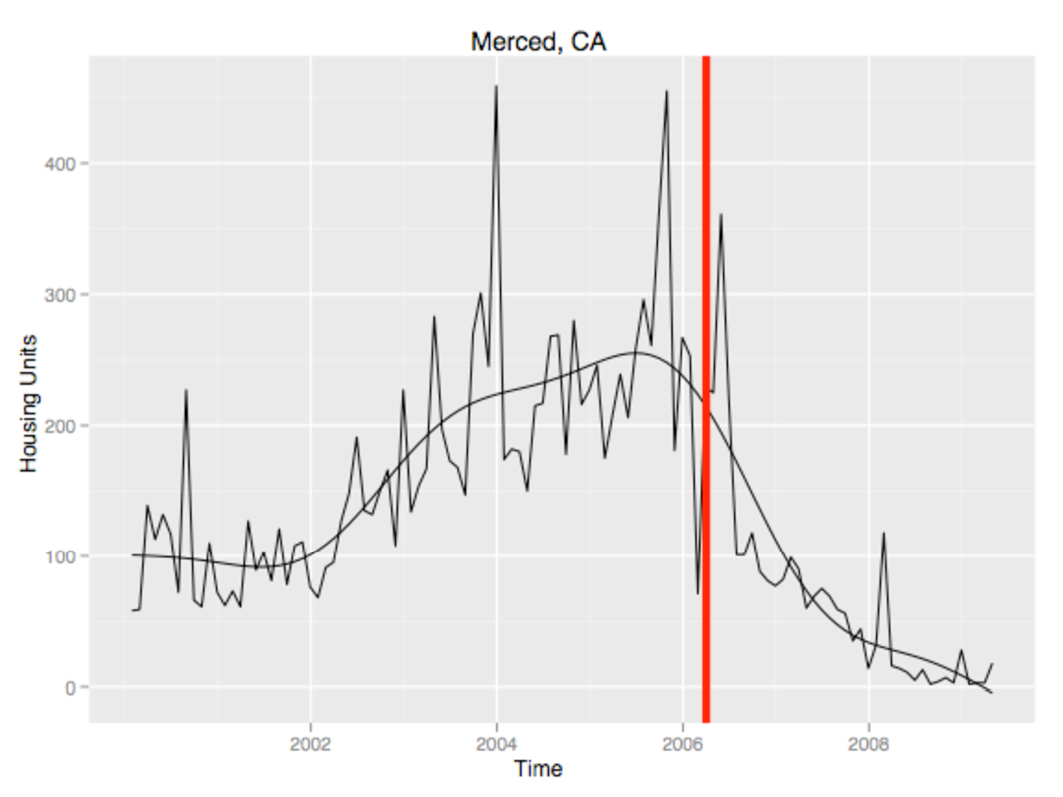
\includegraphics[scale=0.5]{merccon.pdf}
\caption{Total construction of housing units built over time in Merced, California. The red line is the year Merced�s HPI peaked.}
\label{fig:merccon}
\end{centering}
\end{figure}

\subsection{Myth Busters}
After discovering Merced, CA we decided to look more closely at college towns. Contrary to belief, college towns were not greatly impacted by the housing crisis.  They were affected more by the location that they were in, rather than being a ``college town''. (Fig \ref{fig:college})

\begin{figure}[htp]
\begin{centering}
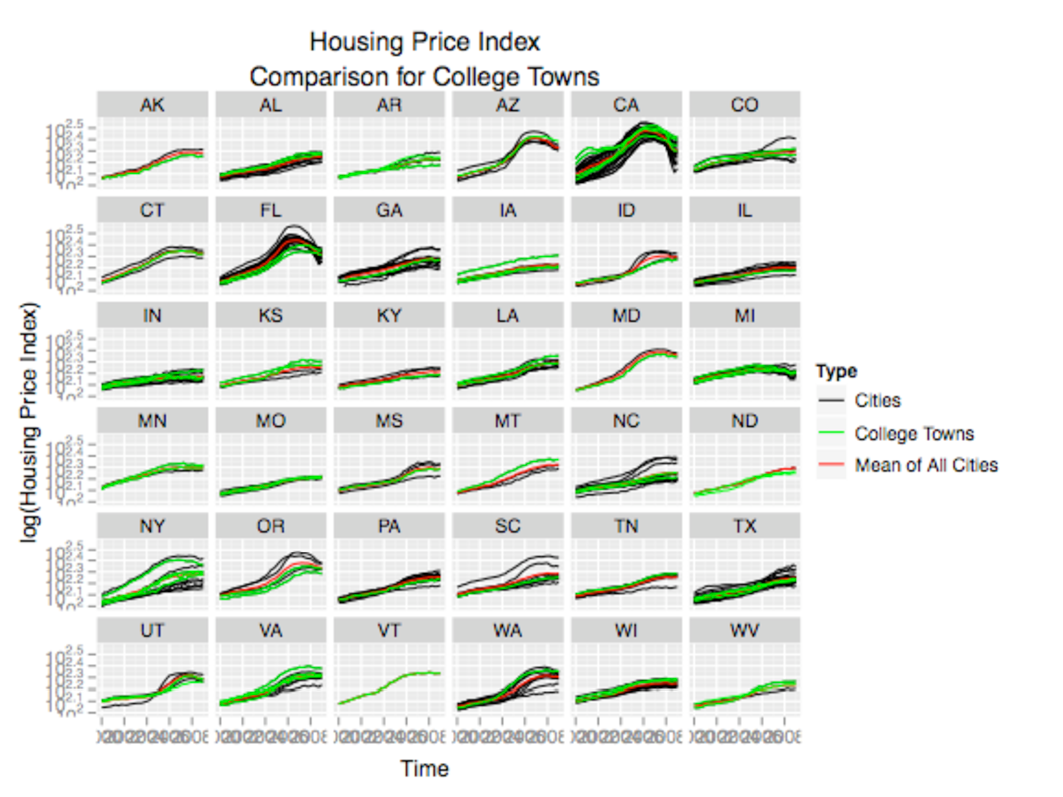
\includegraphics[scale=0.5]{college.pdf}
\caption{HPI for cities, college towns, and the average. Besides a few special cases, the HPI for college towns seem to fall close to the average HPI.}
\label{fig:college}
\end{centering}
\end{figure}



\section{Other Explorations}

\begin{itemize}
\item \textbf{Vacation Spots:} 

Are areas where people own a second home more affected?

\item \textbf{Renting vs. Owning:} 

Is is better to rent or own a house?

\item \textbf{Migration:} 

Are cities that experienced massive population change affected?

\item \textbf{Gross Domestic Product:} 

Can we categorize a certain city by industry? 

Is there a relationship between cities that were hit by the housing crisis?

\end{itemize}

\section{Communication and Future Work}
It is extremely important that all of our data cleaning and findings are reproducible. We've made both the data and programming code available to the public through our PFUG's website on \htmladdnormallink{Gihhub}{http://github.com/hadley/data-housing-crisis/tree/master}. Github is a very advance website that is able to track changes made to data and code from multiple individuals. 

Github is advantageous to both our research group and to the general public. Firstly, we are able to freely store large amounts of data. Also it allows us to work on the same data without having to e-mail changes back and forth. In addition, others can view and download our data for free.  We hope that by keeping the code transparent and self-replicating, others are able to easily build off our work. 

We would like to develop a website that will allow users to easily access the data they are interested in, which would otherwise be a daunting task for those who wish to use a data set of this size. Because our analysis and findings also involve large amounts of information, (such as construction price time series for each US metropolitan area) we are exploring interactive graphical methods for displaying this information. Our future research will involve using the internet application \htmladdnormallink{ManyEyes}{http://manyeyes.alphaworks.ibm.com/} and then eventually the program \htmladdnormallink{Protovis}{http://vis.stanford.edu/protovis/}, to create this website. 


%%%%%%%%%%%%%%%%%%%%%%%%%%%%%%%%%%%%%%%%%%%%%%%%%%%%%%%%%%%%%%%%%%%%%%%%%%%%%%%%
%%%%%%%%%%%%%%%%%%%%%%%%%%%%%%%%%%%%%%%%%%%%%%%%%%%%%%%%%%%%%%%%%%%%%%%%%%%%%%%%
%%%%%%%%%%%%%%%%%%%%%%%%%%%%%%%%%%%%%%%%%%%%%%%%%%%%%%%%%%%%%%%%%%%%%%%%%%%%%%%%
%%%%%%%%%%%%%%%%%%%%%%%%%%%%%%%%%%%%%%%%%%%%%%%%%%%%%%%%%%%%%%%%%%%%%%%%%%%%%%%%
%%%%%%%%%%%%%%%%%%%%%%%%%%%%%%%%%%%%%%%%%%%%%%%%%%%%%%%%%%%%%%%%%%%%%%%%%%%%%%%%
%%%%%%%%%%%%%%%%%%%%%%%%%%%%%%%%%%%%%%%%%%%%%%%%%%%%%%%%%%%%%%%%%%%%%%%%%%%%%%%%
%%%%%%%%%%%%%%%%%%%%%%%%%%%%%%%%%%%%%%%%%%%%%%%%%%%%%%%%%%%%%%%%%%%%%%%%%%%%%%%%
%%%%%%%%%%%%%%%%%%%%%%%%%%%%%%%%%%%%%%%%%%%%%%%%%%%%%%%%%%%%%%%%%%%%%%%%%%%%%%%%
%%%%%%%%%%%%%%%%%%%%%%%%%%%%%%%%%%%%%%%%%%%%%%%%%%%%%%%%%%%%%%%%%%%%%%%%%%%%%%%%
%%%%%%%%%%%%%%%%%%%%%%%%%%%%%%%%%%%%%%%%%%%%%%%%%%%%%%%%%%%%%%%%%%%%%%%%%%%%%%%%
%\section{OLD STUFF}
%\subsection{Purpose of the Template}
%The present template is designed to provide very rudimentary
%guidance on how to write LaTeX source that can easily be 
%converted into Connexions.  Here we use only one add-on packages,
%\verb|graphicx|, which we use to include graphics.
%A number of additional packages are also supported; see 
%\verb|http://www-sop.inria.fr/apics/tralics/packages.html|.
%Given the importance of citing one's sources in research work,
%we also include bibliography references in this file.
%
%This small document makes no effort to teach basic LaTeX skills.  
%Many resources are available for this,
%such as the fundamental book by Lamport~\cite{Lam94}.
%Donald Knuth, the author of the underlying TeX program,
%provides a treasure-trove of information not only about
%the technical aspects of TeX, but also about good mathematical
%typesetting style~\cite{Knu86}.
%
%%%%%%%%%%%%%%%%%%%%%%%%%%%%%%%%%%%%%%%%%%%%%%%%%%%%%%%%%%%%%%%%%%%%%%%%%%%%%%%%%
%\subsection{General Instructions for Conversion}
%
%Connexions provides online instructions that guide you through the
%process of uploading your LaTeX source files.  At present, you must
%use the Firefox or Internet Explorer browsers to properly view and edit
%Connexions content.
%To upload files, you will also need to create your own Connexions account;
%see \verb|http://cnx.org/join_form| for details.
%
%To convert your LaTeX document, you first need to create a \verb|.zip|
%file that contains your \verb|.tex| source files, 
%your \verb|.bib| file if you have a bibliography, 
%and any image files you include in your document.
%Note: the names of your LaTeX source file and zip file must have the
%same stem.  For example, \verb|foo.tex| should be packaged into \verb|foo.zip|.
%Now log-in to Connexions, go to your Workspace,
%create a new module with MathML support, and fill-in the basic
%``Metadata,'' such as the title and summary.  (The top of this LaTeX 
%template contains some a basic text for the Summary: please copy, paste,
%and manually edit this text in the Summary box.) 
%Finally, you arrive at the ``Edit Text'' window, with options to 
%import from various file formats.  Choose ``LaTeX'', and then select 
%the \verb|.zip| file that contains your source files.  Connexions
%commences with the conversion procedure, and in a few moments
%you should be presented with a translated version of your 
%LaTeX document, in a format that allows for further edits
%directly in Connexions.
%You should proof-read the conversion to make sure all text
%and equations appear as you intended.  
%When satisfied, you can preview and publish your document.
%
%
%
%%%%%%%%%%%%%%%%%%%%%%%%%%%%%%%%%%%%%%%%%%%%%%%%%%%%%%%%%%%%%%%%%%%%%%%%%%%%%%%%%
%\section{Rules for Converting LaTeX Source}
%
%Connexions generally does a fine job translating LaTeX source
%code into the native Connexions mark-up language.  
%However, one may need to adapt one's usual typesetting habits
%to work around a few idiosyncrasies. 
%Firstly, one should not invest effort in adjusting page margins,
%line spacing, and fonts: the converter will strip away much of
%this veneer and replace it with the standard Connexions stylings.
%Equations will not be converted into graphics (as is common 
%in LaTeX to HTML conversion), but will rather be translated
%into MathML fonts that can be subsequently edited in Connexions.
%Do not include a title or abstract in your LaTeX document: these 
%must be entered into Connexions manually when you set up your module.
%
%The Connexions converter will not properly handle several LaTeX commands,
%as noted in the online help
%({\tt http://cnx.org/help/UsingLaTeX}).
%\begin{itemize}
%\item The \verb|\mbox| command is not supported.
%\item Nested tables are not supported.
%\item LaTeX allows functions like \verb|\sqrt| to be followed by a 
%      single argument without brackets, e.g., \verb|\sqrt\pi|.
%      The Connexions translator misses this syntax; one instead
%      needs to use brackets \verb|\sqrt{\pi}|.
%\end{itemize}
%
%%%%%%%%%%%%%%%%%%%%%%%%%%%%%%%%%%%%%%%%%%%%%%%%%%%%%%%%%%%%%%%%%%%%%%%%%%%%%%%%%
%\subsection{Future Editing}
%
%You will likely want to make changes to your file at some point after you
%have uploaded the LaTeX document into Connexions.  
%Should you edit the LaTeX document, then re-import, or should you
%alter the code directly in Connexions? 
%If you have major mathematical edits, it may well be easiest to directly
%alter the LaTeX source.  Beware that when you upload, any changes that 
%you made to the previous version directly in Connexions will be overwritten.
%This is not such a concern if you can make all the edits you desire
%directly in LaTeX; however, this is not always the case: some things
%must be done in Connexions.  (For example, see the comments about 
%the \verb|verbatim| environment in Section~\ref{sec:code} below.)
%
%%%%%%%%%%%%%%%%%%%%%%%%%%%%%%%%%%%%%%%%%%%%%%%%%%%%%%%%%%%%%%%%%%%%%%%%%%%%%%%%%
%\subsection{Importing Equations}
%
%We list a few sample equations to test the ability of the converter.
%For example, we have the Pythagorean Theorem, $a^2 + b^2 = c^2$.
%This is an example of an \emph{inline} equation, as is the integral
%$\int_0^\infty e^{-x^2} \, dx$. 
%The same integral can also be typeset as a \emph{displayed} equation,
%\[ \int_0^\infty e^{-x^2} \, dx.\]
%To typeset a matrix, use the LaTeX \verb|array| environment:
%\[ A = \left[ \begin{array}{cc} a & b \\ c & d \end{array}\right].\]
%(Note that the TeX \verb|\matrix| command does not properly translate.)
%
%%%%%%%%%%%%%%%%%%%%%%%%%%%%%%%%%%%%%%%%%%%%%%%%%%%%%%%%%%%%%%%%%%%%%%%%%%%%%%%%%
%\subsection{A sample figure}
%
%Figure~\ref{fig:gap} shows the gap between consecutive
%prime numbers; see~\cite{Hux71}.
%Beware: though the original image was drawn in precise vector graphics, the
%converter has turned it into a bitmap of substantially diminished quality.
%Make sure you make your fonts large enough that they remain legible after
%the translation (unlike this figure).  
%The translator also seems to place the figure directly after the reference,
%so the location of the figure in your Connexions document will generally
%differ from its placement in your LaTeX document (often for the better).
%Notice that if you choose the print the Connexions module as a \verb|.pdf|
%file, the output will include the bitmapped image, rather than the sharp
%version in your original document.
%
%\begin{figure}
%\begin{center}
%%\includegraphics[scale=0.5]{prime_gap}
%\end{center}
%\caption{\label{fig:gap}
%   The gap between consecutive prime numbers.}
%\end{figure}
%
%%%%%%%%%%%%%%%%%%%%%%%%%%%%%%%%%%%%%%%%%%%%%%%%%%%%%%%%%%%%%%%%%%%%%%%%%%%%%%%%%
%\subsection{A sample table}
%
%Table~\ref{tbl:mersenne} provides a list 
%of the first seven Mersenne primes.
%(Beware: The Converter does not properly handle
%the caption command for tables.  For example,
%if a caption precedes the table itself, as is the usual custom,
%the reference does not translate properly.  
%Moreover, Connexions seems to draw boxes around all cells,
%regardless of the formatting in the LaTeX source.)
%
%\begin{table} 
%\begin{center}
%\begin{tabular}{r|ccccccc}
%$k$                  & 1 & 2 & 3  & 4   & 5    & 6      & 7 \\ \hline 
%$k$th Mersenne prime & 3 & 7 & 31 & 127 & 8191 & 131071 & 524287
%\end{tabular}
%\end{center}
%\caption{\label{tbl:mersenne}
%         Mersenne primes.}
%\end{table}
%
%%%%%%%%%%%%%%%%%%%%%%%%%%%%%%%%%%%%%%%%%%%%%%%%%%%%%%%%%%%%%%%%%%%%%%%%%%%%%%%%%
%\subsection{Incorporating code} \label{sec:code}
%
%You might naturally want to include small snippets of code with your report,
%which you would incorporate in LaTeX using the \verb|verbatim| environment.
%For example, the following MATLAB commands produce the Mersenne prime data
%given in Table~\ref{tbl:mersenne}.
%
%\begin{verbatim}
%  p=[1:20]';
%  pmer = p(isprime(2.^p-1)); 
%  disp([[1:length(pmer)]' 2.^pmer-1])
%\end{verbatim}
%
%At present, the Connexions LaTeX translator does not properly handle
%the \verb|verbatim| environment, though this is expected to improve 
%in an updated translator that will be available in a few months.
%In the meantime, it is best to leave code out of your LaTeX document, 
%and paste it into Connexions manually as a \verb|<code>| block.
%
%%%%%%%%%%%%%%%%%%%%%%%%%%%%%%%%%%%%%%%%%%%%%%%%%%%%%%%%%%%%%%%%%%%%%%%%%%%%%%%%%
%\subsection{Adding a Bibliography}
%
%Connexions works well with LaTeX's bibliography tool, BibTeX.
%This tool allows you to create a \verb|.bib| file that contains
%a database of papers and books that you regularly reference.  
%For example, this template is accompanied by a file called 
%\verb|mybibfile.bib| that contains the three references 
%cited here.  
%You add citations in your LaTeX document using the 
%\verb|\cite| command.  See Lamport~\cite{Lam94} for details.
%
%%%%%%%%%%%%%%%%%%%%%%%%%%%%%%%%%%%%%%%%%%%%%%%%%%%%%%%%%%%%%%%%%%%%%%%%%%%%%%%%%
%% Please leave this Acknowlegement to VIGRE in your modules
%%%%%%%%%%%%%%%%%%%%%%%%%%%%%%%%%%%%%%%%%%%%%%%%%%%%%%%%%%%%%%%%%%%%%%%%%%%%%%%%
\section{Acknowledgements}

This Connexions module describes work conducted as part of Rice 
University's VIGRE program, supported by National Science Foundation
grant DMS--0739420.


\end{document}
